\newpage
\section{Results}
% General structure.
%   Display chip structure
% 	Display spectrums, try to calculate quality factor at least.
%   Display some prelimary purities.

% Some stuff I probably should have calculated:
% Powers in the waveguide, peak power
\subsection{Glassgow}



This chip was used to do an initial proof of concept that the JSI of a ring resonator could be measured. Here the aim was to simply see how the experiment compared to the simulation and theory already existing.

A Pritel pulsed laser was used with <2ps 1.0nm 1530-1560 >100 W


\begingroup
    \centering  
    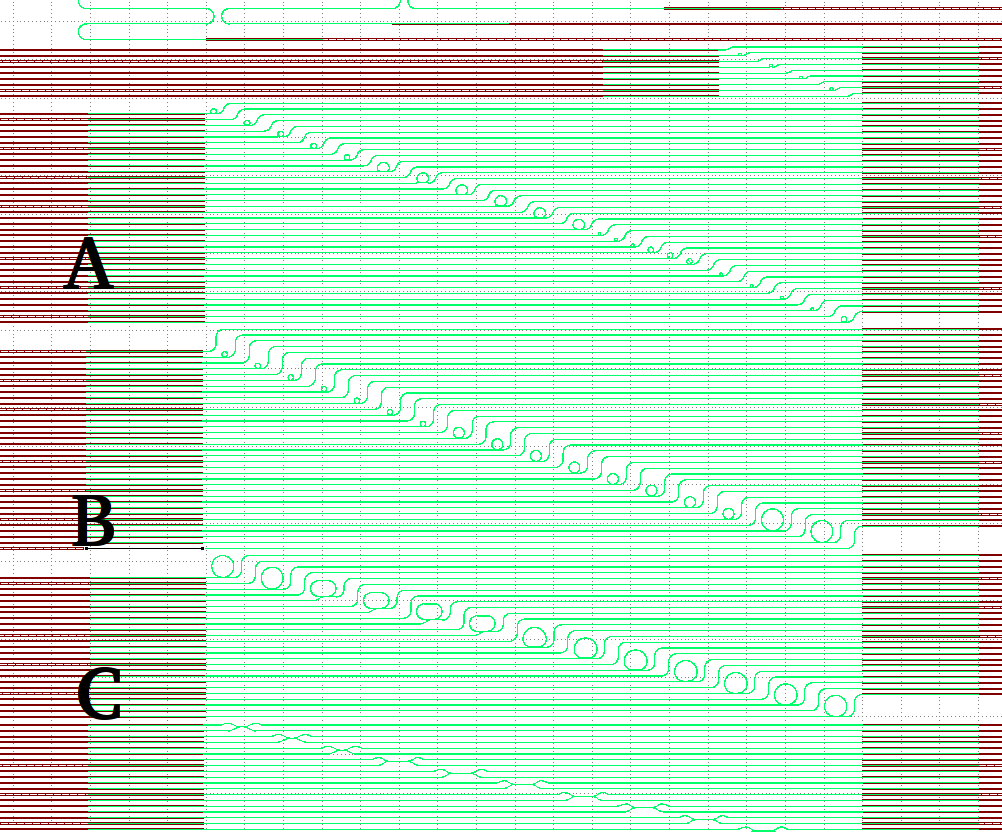
\includegraphics[width=10cm]{img/results/glassgowChipNumbering.png}
    \captionof{figure}{Glassgow test structure chip}
     \vspace{3pt} \label{crossCompare}
\endgroup

% Display some joint spectrums. Estimate the power you were putting into the ring. 

\subsection{Toshiba}
\begingroup
    \centering  
    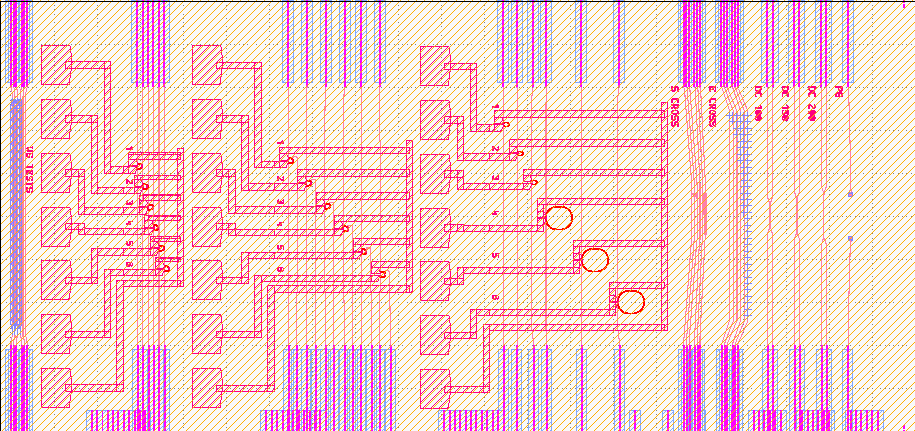
\includegraphics[width=10cm]{img/results/toshiba.png}
    \captionof{figure}{Glassgow test structure chip}
     \vspace{3pt} \label{crossCompare}
\endgroup

\subsubsection{Bistability Data}
% Should be easy
\subsubsection{Pulse shaping}
% Touch on the pulse shaping experiment
\subsubsection{Power Scans}
%
\subsection{a-Si}
\begingroup
    \centering  
    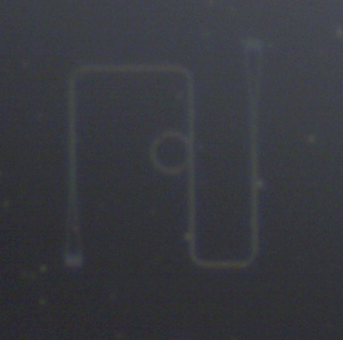
\includegraphics[width=10cm]{img/results/chipPictures/exampleASIRing.png}
    \captionof{figure}{Glassgow test structure chip}
     \vspace{3pt} \label{crossCompare}
\endgroup
% Some initial joint spectrums.
% Try to calculate the quality of the rings.
% Analyse the g2(0) data